\section{Zielsetzung}
Ziel des Versuches ist es, mit Hilfe der Debye-Scherrer Methode, Eigenschaften
über Strukturen von Metallen und Salzen zu ermitteln. Innerhalb dieses
Versuches wurde mittels der Debye-Scherrer Aufnahmen Rückschlüsse über die
Netzebenabstände und die Struktur der Elementarzellen geschlossen.


\section{Theorie}
\label{sec:Theorie}
Die zu untersuchende Materie weißt kristalline Strukturen auf, sodass zuerst
innerhalb der Theorie auf die verschiedenen Kristallstrukturen eingegangen wird.\\
\subsection{Grundlagen zur Kristallstrukturen}
Kristalle bestehen aus einer periodisch angeordneten Basis, welche für
verschiedene Kristalle aus einem oder mehreren Atomen bestehen kann.
Die Form und die periodische Anordnung im Raum legen fest,
was für eine Kristallstruktur vorliegt. \\
Durch die Translation der Basisvektoren in jede Richtung des Raumes
,kann jeder Punkt des Gitters durch eine Linearkombination $\vec l$
der Basisvektoren dargestellt werden.
$$ \vec l = n_1 \vec a + n_2 \vec b + n_3 \vec c .$$
Die Faktoren $n_1-n_3 $
Abbildung
\begin{figure}
    \centering
    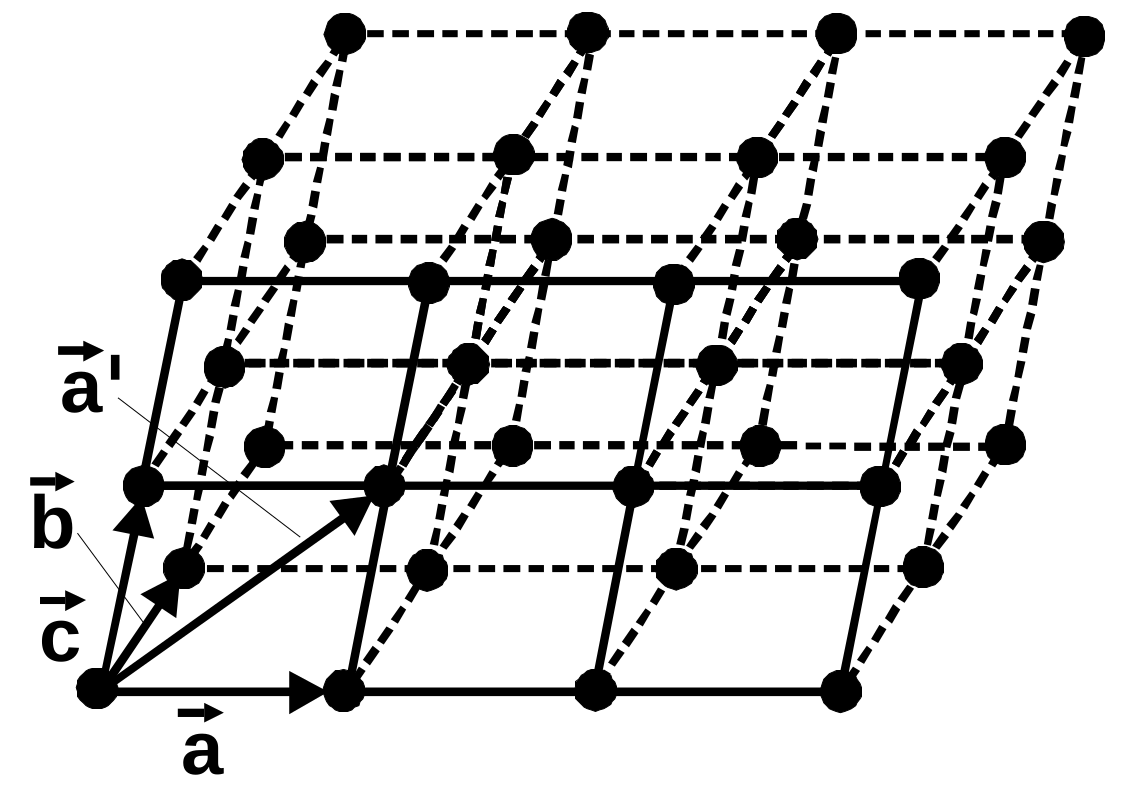
\includegraphics[width=0.55\textwidth]{ressources/gitter.png}
    \caption{Eines Gitters mit verschiedenen Gitterpunkten und deren mögliche
    Verschiebung durch den Translationsvektor $\vec l$\cite{skript}.}
    \label{fig_gitter}
\end{figure}
\ref{fig_gitter}
 stellt eine mögliche Anordnung eines Gitters mit
einer einatomigen Basis dar (Punktgitter). Jeder Punkt des Gitters kann von
jedem Punkt durch die Linearkombination $\vec l$ erreicht werden.

\subsection{Elementarzelle}

Eine Elementarzelle definiert die kleinste Einheit einer Kristallstruktur.
Es wird zwischen primitive Einheitszellen und Einheitszellen mit mehreren Atomen
(z.B. Salze) unterschieden. Im Fall einer primitiven Einheitszelle
liegt auf jeder Ecke der Einheitszelle das gleiche Atom. Das heißt die Gitterpunkte
bilden gleichzeitig auch das Kristallgitter. In der Abbildung \ref{primitiv} ist
eine kubisch primitive Einheitszelle dargestellt, um einen beliebig gewählten Eckpunkte kann
eine primitive Einheitszelle festgelegt werden.

\begin{figure}
    \centering
    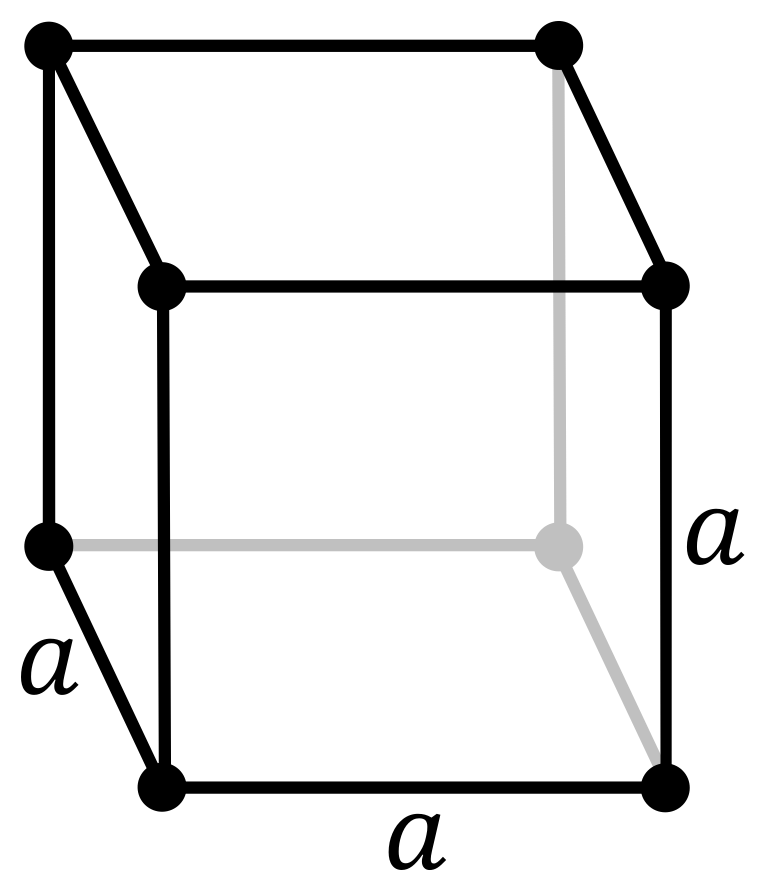
\includegraphics[width=0.25\textwidth]{ressources/primitiv.png}
    \caption{Kubisch primitives Gitter\cite{skript}.}
    \label{primitiv}
\end{figure}
Nicht jedes Gitter kann durch primitive Einheitszellen aufgebaut werden.
Ist dieses der Fall so besitzt die Einheitszellen mehreren Atomen.
Ein Beispielt hierfür ist die Einheitszelle von Natriumchlorid ($\text{Na}^+\text{Cl}^-)$,
wobei die Einheitszelle aus Na$^+$ und Cl$^-$- Ionen besteht.
\subsection{Kristalline Strukturen}

Die mögliche Anzahl an Gitterstrukturen ist durch die drei Dimensionen beschränkt und
wird durch die 14 Bravais-Gitter wiedergegeben. Diese lassen sich anhand
Einheitszellen in sieben verschiedene Gittertypen einordnen. Im folgenden
wird auf die kubischen Gitterstrukturen weiter eingegangen.
\subsubsection{Kubische Gitterstrukturen}
Die kubische Gitterstruktur wird innerhalb der Bravais-Gitter in drei
verschiedene Gitterstrukturen aufgeteilt. Die verschiedene kubischen Strukturen
sind in den Abbildungen \ref{primitiv}- \ref{bcc} dargestellt.

\begin{figure}
    \centering
    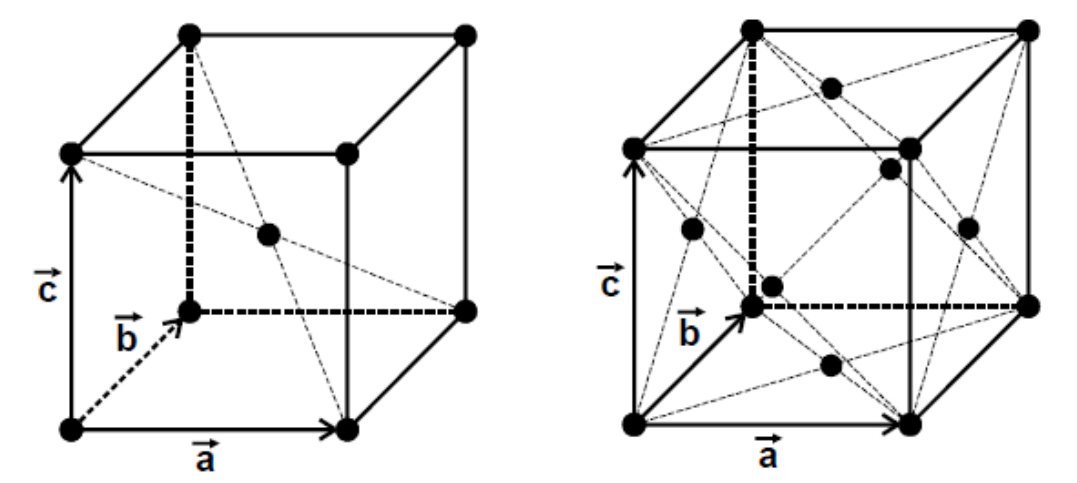
\includegraphics[width=0.55\textwidth]{ressources/kubies.png}
    \caption{Abbildung eines bcc-Gitters (links) und eines fcc-Gitters\cite{skript}.}
    \label{bcc}
\end{figure}

Das kubisch primitive Gitter besitzt wie in Kapitel 2.2 erwähnt eine
primitive Einheitszelle mit einem Atom in $1/8$ in jeder Würfelecke.
Wenn man dieses als Koordinaten der Punkte der Basis
schreibt, erhält man für die primitive Einheitszelle:
$$ (\,0,\,0,\,0).$$
Das kubisch raumzentierte Gitter, vgl. Abbildung \ref{bcc}, besitzt eine Basis mit 2 Atomen,
eines in der Würfelecke und eines in der Mitte jedes Würfels. Schreibt man
die Koordinaten dieser Basis auf so ergibt sich:
$$(\,0\,,\,0\,,\,0\,) \quad (\,\frac{1}{2}\,, \,\frac{1}{2}\, ,\, \frac{1}{2}\,)$$
Das kubisch flächenzentrierte Gitter ist das komplexeste der drei kubischen Bravais-Gitter.
Dieses besitzt auf jeder der sechs Würfelseiten ein weiteres Atom. Die damit
verbundene Basis hat 4 Atome. Weißt man ihnen Koordinaten zu so ergibt sich
für diese Basis:
$$(\,0,\,0,\,0), \quad (\,\frac{1}{2},\, \frac{1}{2} ,\, 0), \quad (\, \frac{1}{2}, \,0 ,\, \frac{1}{2}),
\quad (\,0, \, \frac{1}{2} , \, \frac{1}{2}).$$
Innerhalb des Versuches werden die Proben auf verschiedene kubische Strukturen
untersucht, welche sich aus mehreren kubischen Bravais-Gitter zusammensetzen.
Die Diamantstruktur lässt sich aus zwei kubisch flächenzentrierten Gitter
zusammensetzen, wobei das zweite kubisch flächenzentrierte Gitter um
$\frac{1}{4}$ in einer Raumdiagonalen verschoben ist. Die daraus folgende
Basis besitzt 8 Atome. Die ersten 4 sind die des einfach flächenzentrierten
kubischen Gitters:

$$(\,0,\,0,\,0), \quad (\,\frac{1}{2},\, \frac{1}{2} ,\, 0), \quad (\, \frac{1}{2}, \,0 ,\, \frac{1}{2}),
\quad (\,0, \, \frac{1}{2} , \, \frac{1}{2}).$$
Die Weiteren 4 sind die jeweils um die Raumdiagonalen verschobenen Atome:
$$ (\, \frac{1}{4},\, \frac{1}{4}, \, \frac{1}{4}), \quad (\frac{3}{4}, \, \frac{3}{4}, \, \frac{1}{4}),
\quad (\, \frac{3}{4}, \, \frac{1}{4}, \frac{3}{4}), \quad (\,\frac{1}{4},\,  \frac{3}{4}, \, \frac{3}{4}) $$
Die Zinkblende-Struktur ist ähnlich zur Diamantstruktur, nur dass diese aus
Zink und Schwefel Atomen besteht. Jedes der beiden Untergitter
ist mit ausschließlich Schwefel oder Zink Atomen besetzt.\\
Bei der Steinsalz-Struktur besteht das Gitter aus zwei versetzten kubisch-flächenzentrierten
kubischen Gittern, welche um eine halbe Raumdiagonale verschoben sind. Die
Positionen der Atome einer Einheitszelle liegen bei:
\begin{align}
    A:(\,0,\,0,\,0), \quad (\,\frac{1}{2},\, \frac{1}{2} ,\, 0), \quad (\, \frac{1}{2}, \,0 ,\, \frac{1}{2}),
    \quad (\,0, \, \frac{1}{2} , \, \frac{1}{2}) \\
    B:(\,\frac{1}{2},\,\frac{1}{2},\,\frac{1}{2},, \quad (\,1 , \, 1 , \quad\frac{1}{2},)
    ,\quad (1, \,\frac{1}{2}, \,1),\quad (\,\frac{1}{2}, \, 1, \,1.)
\end{align}
Die Gitterstruktur von Cäsiumchlorid besteht ebenfalls aus zwei unterschiedlichen
kubisch-primitiven Gittern, welche ebenfalls um eine halbe Raumdiagonale
verschoben sind. Die Posiotionen der zweiatomigen Basis aus Cäsium und Chlor liegt bei:
\begin{align}
A:(\,0 , \, 0 , \, 0)\\
B:(\, \frac{1}{2},\, \frac{1}{2},\, \frac{1}{2})
\end{align}
\subsection{Millersche Indices}

Die Millerschen Indices dienen dazu eine Netzebene eines Kristalles und deren
Lage im Raum genauer zu beschreiben. Die millerschen Indices bestehen aus einen Zahlentripel
(h,k,l). Jeder dieser Indices gibt den reziproken Wert der Schnittpunkte der
Netzebene mit den Achsenabschnitten an. Mit den Millerschen Indices lässt sich der
Netzabstand zweier Ebenen berechnen. Die Netzebenen die parallel zu einandner
liegen bilden eine Netzebenenschar. Der Abstand zweier Netzebenen lässt sich
durch die Millerschen Indices ausdrücken:
$$ d=\frac{1}{\sqrt{
\left(\frac{h}{a} \right)^2 + \left(\frac{k}{b} \right)^2 + \left(\frac{l}{c} \right)^2.
}}
$$
Für die kubischen Gitterstrukturen vereinfacht sich der allgemeine Zusammenhang zu:
\begin{align}
d=\frac{a}{\sqrt{h^2 + k^2 + l^2}}
\label{gitti}
\end{align}
\subsection{Beugung von Röntgenstrahlung an Kristallen}
Trifft Röntgenstrahlung auf einen Kristall, beziehungsweise auf die Elektronen
und die Atome, so kann die Wechselwirkung  als ein klassischer Streuprozess
aufgefasst werden. Die innerhalb des Streuprozesses angeregten geladenen
Teilchen emittieren Strahlung, wobei in Abhängigkeit des Kristallgitters
bestimmte Interferenzeffekte auftreten. Die Schwingungen der angeregten
geladenen Teilchen können als Hertzscher Dipol aufgefasst werden.
Aufgrund der Eigenschaften des Hertzschen Dipols kann ein
Zusammenhang zwischen der Intensität der emittierten Strahlung und
der Masse $m$ des schwingenden Teilchens angegeben werden.
Dabei wird effektiv nur an den Elektronen in den Atomhüllen gestreuut.
$$I \approx \frac{1}{m^2}$$

Der naive Ansatz ist, dass die emittierte Strahlung des
Atoms $I_a$ proportional zur Ordnungszahl $z$ ist.
Da die Elektronenhülle der Atome eine endliche Ausdehnung besitzt und
es somit zu einer Phasendifferenz, zwischen Elektronen die an
"Anfang" und "Ende" der Elektronenhülle wechselwirken kommt,  sinkt die
Intensität. Dieser Effekt wird durch den Atomformfaktor $f$ ,welcher
materialabhängig ist, beschrieben. Die Intensität $I_a$ verglichen mit
der Intensität, welche durch eine Streuung an einem einzelnen Elektron ensteht,
ergibt:
\begin{align}
    f^2\left( \frac{\sin \theta}{\lambda}Z \right)=\frac{I_a}{I_e}
    \label{atom}
\end{align}
Der Atomformfaktor hängt vom Winkel $\theta$, der Ordnungszahl $z$ und der
Wellenlänge $\lambda$ ab, das Ziel ist die Berechnung der Phasendifferenz zweier
Wellen, welche an unterschiedlichen Orten gestreut werden.
In der Abbildung \ref{bragg} ist eine schematische Skizze zur
Berechnung der Phasendifferenz dargestellt.
\begin{figure}
    \centering
    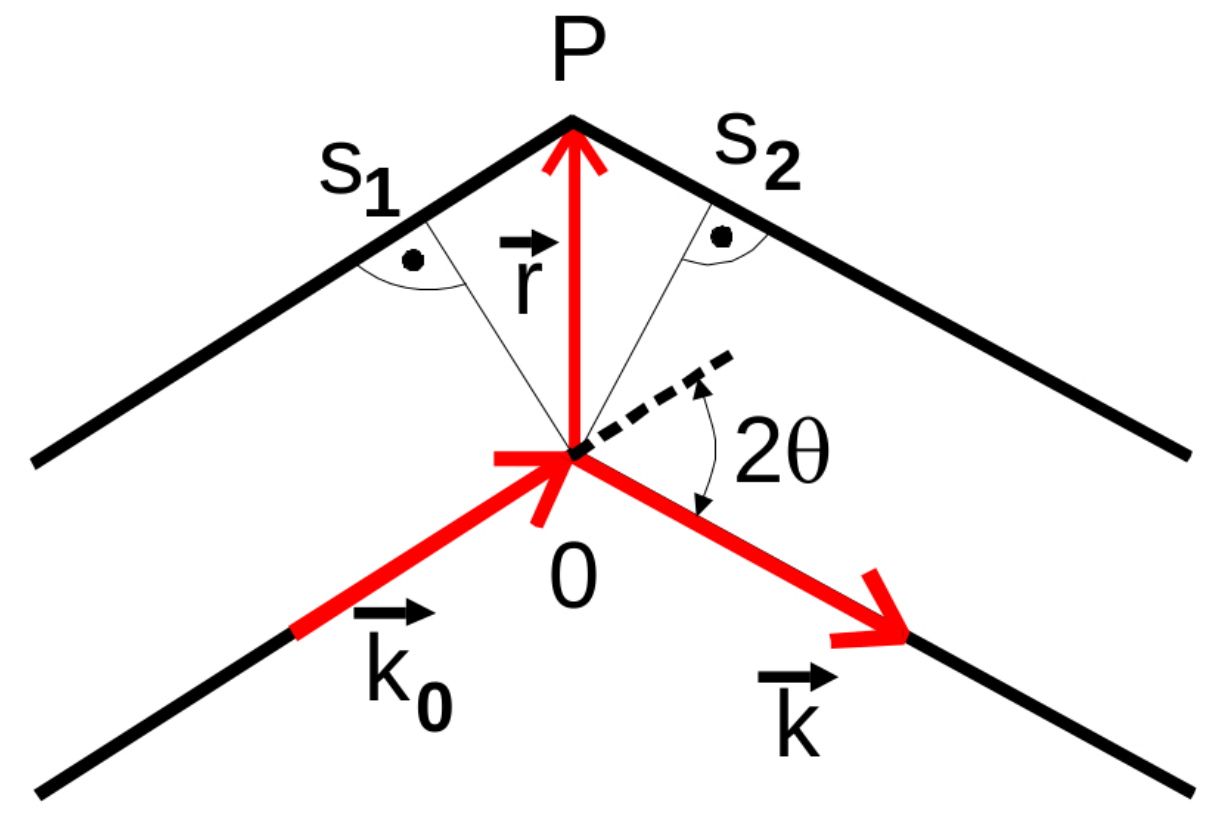
\includegraphics[width=0.55\textwidth]{ressources/bragg.png}
    \caption{Skizze zur Berechnung der Phasendifferenz\cite{skript}.}
    \label{bragg}
\end{figure}
Für die einfallenden ($|\vec{k}|$) und gestreuten Wellenvektoren $|\vec{k_0}|$ gilt:
\begin{align}
|\vec{k}|=|\vec{k_0}|=\frac{1}{\lambda}
    \label{welle}
\end{align}
Mit Hilfe des Wellenvektors lässt sich der Gangunterschied $\Delta s$ zwischen
zwei Wellen, welche an den Punkten 0 und P gestreut werden, berechnen

\begin{align}
    \Delta s= s_1 + s_2= \vec{r} \left(\frac{\vec{k}}{k}-\frac{\vec{k_0}}{k_0} \right).
\end{align}
Damit folgt für die Phasendifferenz $\Delta \Phi$:
\begin{align}
     \Delta \Phi= 2\pi \frac{\Delta s}{\lambda}= 2 \pi \vec{r}\cdot(\vec{k}-\vec{k_0}).
\end{align}
Die Streuamplitude, welche nachher für die Ringe auf den Debye-Scherrer Aufnahmen
verantwortlich sind, ergeben sich wenn über alle Positionen der Atome $r_i$
innerhalb einer Einheitszelle summiert wird
\begin{align}
A=\sum_j f_j e^{-2 \pi i \vec{r_j} (\vec{k}-\vec{k_0})} I_e=\sum_j f_j e^{-2\pi i (x_j\vec{a}
+y_j \vec{b} + z_j \vec{c})(\vec{k}-\vec{k_0})} I_e
\end{align}
Gegeben sei die Bragg Bedingung:
\begin{align}
n\lambda = 2d \sin \theta
    \label{braggi}
\end{align}
Für den reziproken Raum gilt analog die Laue Bedingung:
\begin{align}
    \vec{g}= \vec{k}-\vec{k_0}= h \vec{A}+ k\vec{B}+l\vec{C}
\end{align}
mit
\begin{align*}
    \vec{A}= \frac{\vec{b} \times \vec{c}} { \vec{a} (\vec{b} \times \vec{c})}\\
    \vec{B}= \frac{\vec{c} \times \vec{a}} { \vec{a} (\vec{b} \times \vec{c})}\\
    \vec{C}= \frac{\vec{a} \times \vec{b}} { \vec{a} (\vec{b} \times \vec{c})}
\end{align*}
Die Streuamplitude $S$ ergit sich mit Hilfe der Gleichungen (9) und (11):
\begin{align}
    S=\sum_j f_j e^{-2 \pi i \vec{r_j} \vec{g}}=\sum_j f_j e^{-2 \pi i(x_j
    h + y_j k + z_j l)}
\label{streu}
\end{align}
Die Streuamplitude ($S(h,k,l)$) hängt nun von den Millerschen Indices $h,k,l$ ab,
das heißt es lässt sich für die Netzebenen berechnen, ob ein Reflex sichtbar ist oder nicht.
% 2x2 Plot
% \begin{figure*}
%     \centering
%     \begin{subfigure}[b]{0.475\textwidth}
%         \centering
%         \includegraphics[width=\textwidth]{Abbildungen/Schaltung1.pdf}
%         \caption[]%
%         {{\small Schaltung 1.}}
%         \label{fig:Schaltung1}
%     \end{subfigure}
%     \hfill
%     \begin{subfigure}[b]{0.475\textwidth}
%         \centering
%         \includegraphics[width=\textwidth]{Abbildungen/Schaltung2.pdf}
%         \caption[]%
%         {{\small Schaltung 2.}}
%         \label{fig:Schaltung2}
%     \end{subfigure}
%     \vskip\baselineskip
%     \begin{subfigure}[b]{0.475\textwidth}
%         \centering
%         \includegraphics[width=\textwidth]{Abbildungen/Schaltung4.pdf}    % Zahlen vertauscht ... -.-
%         \caption[]%
%         {{\small Schaltung 3.}}
%         \label{fig:Schaltung3}
%     \end{subfigure}
%     \quad
%     \begin{subfigure}[b]{0.475\textwidth}
%         \centering
%         \includegraphics[width=\textwidth]{Abbildungen/Schaltung3.pdf}
%         \caption[]%
%         {{\small Schaltung 4.}}
%         \label{fig:Schaltung4}
%     \end{subfigure}
%     \caption[]
%     {Ersatzschaltbilder der verschiedenen Teilaufgaben.}
%     \label{fig:Schaltungen}
% \end{figure*}
